\documentclass[12pt]{article}
\usepackage[letterpaper, left=13mm, right=13mm, top=20mm, bottom=20mm,
  headheight=15pt, headsep=5mm, footskip=10mm]{geometry}
\usepackage[T1]{fontenc}
\usepackage[utf8]{inputenc}
\usepackage{tgheros}
\renewcommand{\familydefault}{\sfdefault}
\usepackage{fancyhdr}
\usepackage{tikz}
\usetikzlibrary{arrows.meta}
\pagestyle{fancy}
\fancyhf{}
\lhead{\small Week NN / Poisoned cookie / Grades 4--5}
\lfoot{\small Bellingham Math Circle / Week NN / NN-45-v1}
\rfoot{\small \thepage}
\renewcommand{\headrulewidth}{0.4pt}
\renewcommand{\footrulewidth}{0pt}
\setlength{\parindent}{0pt}
\setlength{\parskip}{0pt}
\newcommand{\prob}[1]{\par\textbf{Problem #1:}~}
\raggedright
\begin{document}
Two players take turns. On your turn, put the corner of the bite card on any cookie and eat every cookie under the card. That is the chosen cookie and every cookie above it or to its right, including those up and to the right. Whoever has to eat the poison cookie in the bottom-left corner loses. To record a bite, draw an X on the chosen cookie.\par\vspace{4mm}
{\centering 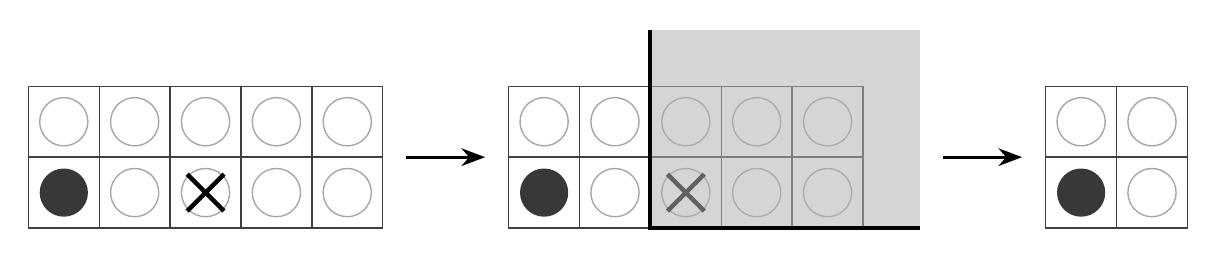
\begin{tikzpicture}[x=1mm, y=1mm]
\draw[line width=0.5pt, black!75] (0,0) rectangle ++(9,9);
\fill[black!78] (4.5,4.5) circle (3.06);
\draw[line width=0.5pt, black!75] (9,0) rectangle ++(9,9);
\draw[line width=0.5pt, black!35] (13.5,4.5) circle (3.06);
\draw[line width=0.5pt, black!75] (18,0) rectangle ++(9,9);
\draw[line width=0.5pt, black!35] (22.5,4.5) circle (3.06);
\draw[line width=0.5pt, black!75] (27,0) rectangle ++(9,9);
\draw[line width=0.5pt, black!35] (31.5,4.5) circle (3.06);
\draw[line width=0.5pt, black!75] (36,0) rectangle ++(9,9);
\draw[line width=0.5pt, black!35] (40.5,4.5) circle (3.06);
\draw[line width=0.5pt, black!75] (0,9) rectangle ++(9,9);
\draw[line width=0.5pt, black!35] (4.5,13.5) circle (3.06);
\draw[line width=0.5pt, black!75] (9,9) rectangle ++(9,9);
\draw[line width=0.5pt, black!35] (13.5,13.5) circle (3.06);
\draw[line width=0.5pt, black!75] (18,9) rectangle ++(9,9);
\draw[line width=0.5pt, black!35] (22.5,13.5) circle (3.06);
\draw[line width=0.5pt, black!75] (27,9) rectangle ++(9,9);
\draw[line width=0.5pt, black!35] (31.5,13.5) circle (3.06);
\draw[line width=0.5pt, black!75] (36,9) rectangle ++(9,9);
\draw[line width=0.5pt, black!35] (40.5,13.5) circle (3.06);
\draw[line width=1.6pt] (20.16,2.16) -- (24.84,6.84) (20.16,6.84) -- (24.84,2.16);
\draw[-{Stealth[length=3mm]}, line width=1pt] (48,9) -- ++(10,0);
\draw[line width=0.5pt, black!75] (61,0) rectangle ++(9,9);
\fill[black!78] (65.5,4.5) circle (3.06);
\draw[line width=0.5pt, black!75] (70,0) rectangle ++(9,9);
\draw[line width=0.5pt, black!35] (74.5,4.5) circle (3.06);
\draw[line width=0.5pt, black!75] (79,0) rectangle ++(9,9);
\draw[line width=0.5pt, black!35] (83.5,4.5) circle (3.06);
\draw[line width=0.5pt, black!75] (88,0) rectangle ++(9,9);
\draw[line width=0.5pt, black!35] (92.5,4.5) circle (3.06);
\draw[line width=0.5pt, black!75] (97,0) rectangle ++(9,9);
\draw[line width=0.5pt, black!35] (101.5,4.5) circle (3.06);
\draw[line width=0.5pt, black!75] (61,9) rectangle ++(9,9);
\draw[line width=0.5pt, black!35] (65.5,13.5) circle (3.06);
\draw[line width=0.5pt, black!75] (70,9) rectangle ++(9,9);
\draw[line width=0.5pt, black!35] (74.5,13.5) circle (3.06);
\draw[line width=0.5pt, black!75] (79,9) rectangle ++(9,9);
\draw[line width=0.5pt, black!35] (83.5,13.5) circle (3.06);
\draw[line width=0.5pt, black!75] (88,9) rectangle ++(9,9);
\draw[line width=0.5pt, black!35] (92.5,13.5) circle (3.06);
\draw[line width=0.5pt, black!75] (97,9) rectangle ++(9,9);
\draw[line width=0.5pt, black!35] (101.5,13.5) circle (3.06);
\draw[line width=1.6pt] (81.16,2.16) -- (85.84,6.84) (81.16,6.84) -- (85.84,2.16);
\fill[black!30, opacity=0.55] (79,0) rectangle (113.2,25.2);
\draw[line width=1.4pt] (113.2,0) -- (79,0) -- (79,25.2);
\draw[-{Stealth[length=3mm]}, line width=1pt] (116.2,9) -- ++(10,0);
\draw[line width=0.5pt, black!75] (129.2,0) rectangle ++(9,9);
\fill[black!78] (133.7,4.5) circle (3.06);
\draw[line width=0.5pt, black!75] (138.2,0) rectangle ++(9,9);
\draw[line width=0.5pt, black!35] (142.7,4.5) circle (3.06);
\draw[line width=0.5pt, black!75] (129.2,9) rectangle ++(9,9);
\draw[line width=0.5pt, black!35] (133.7,13.5) circle (3.06);
\draw[line width=0.5pt, black!75] (138.2,9) rectangle ++(9,9);
\draw[line width=0.5pt, black!35] (142.7,13.5) circle (3.06);
\end{tikzpicture}\par}\vspace{8mm}
\prob{1}On each board, mark a first bite after which the first player can make sure to win.\par\vspace{5mm}
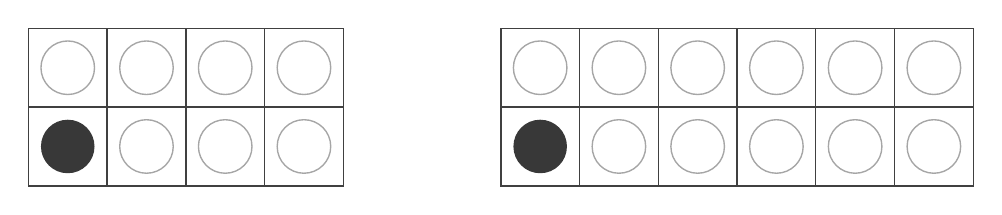
\begin{tikzpicture}[x=1mm, y=1mm]
\draw[line width=0.5pt, black!75] (0,0) rectangle ++(10,10);
\fill[black!78] (5,5) circle (3.4);
\draw[line width=0.5pt, black!75] (10,0) rectangle ++(10,10);
\draw[line width=0.5pt, black!35] (15,5) circle (3.4);
\draw[line width=0.5pt, black!75] (20,0) rectangle ++(10,10);
\draw[line width=0.5pt, black!35] (25,5) circle (3.4);
\draw[line width=0.5pt, black!75] (30,0) rectangle ++(10,10);
\draw[line width=0.5pt, black!35] (35,5) circle (3.4);
\draw[line width=0.5pt, black!75] (0,10) rectangle ++(10,10);
\draw[line width=0.5pt, black!35] (5,15) circle (3.4);
\draw[line width=0.5pt, black!75] (10,10) rectangle ++(10,10);
\draw[line width=0.5pt, black!35] (15,15) circle (3.4);
\draw[line width=0.5pt, black!75] (20,10) rectangle ++(10,10);
\draw[line width=0.5pt, black!35] (25,15) circle (3.4);
\draw[line width=0.5pt, black!75] (30,10) rectangle ++(10,10);
\draw[line width=0.5pt, black!35] (35,15) circle (3.4);
\draw[line width=0.5pt, black!75] (60,0) rectangle ++(10,10);
\fill[black!78] (65,5) circle (3.4);
\draw[line width=0.5pt, black!75] (70,0) rectangle ++(10,10);
\draw[line width=0.5pt, black!35] (75,5) circle (3.4);
\draw[line width=0.5pt, black!75] (80,0) rectangle ++(10,10);
\draw[line width=0.5pt, black!35] (85,5) circle (3.4);
\draw[line width=0.5pt, black!75] (90,0) rectangle ++(10,10);
\draw[line width=0.5pt, black!35] (95,5) circle (3.4);
\draw[line width=0.5pt, black!75] (100,0) rectangle ++(10,10);
\draw[line width=0.5pt, black!35] (105,5) circle (3.4);
\draw[line width=0.5pt, black!75] (110,0) rectangle ++(10,10);
\draw[line width=0.5pt, black!35] (115,5) circle (3.4);
\draw[line width=0.5pt, black!75] (60,10) rectangle ++(10,10);
\draw[line width=0.5pt, black!35] (65,15) circle (3.4);
\draw[line width=0.5pt, black!75] (70,10) rectangle ++(10,10);
\draw[line width=0.5pt, black!35] (75,15) circle (3.4);
\draw[line width=0.5pt, black!75] (80,10) rectangle ++(10,10);
\draw[line width=0.5pt, black!35] (85,15) circle (3.4);
\draw[line width=0.5pt, black!75] (90,10) rectangle ++(10,10);
\draw[line width=0.5pt, black!35] (95,15) circle (3.4);
\draw[line width=0.5pt, black!75] (100,10) rectangle ++(10,10);
\draw[line width=0.5pt, black!35] (105,15) circle (3.4);
\draw[line width=0.5pt, black!75] (110,10) rectangle ++(10,10);
\draw[line width=0.5pt, black!35] (115,15) circle (3.4);
\end{tikzpicture}\par\vspace{10mm}
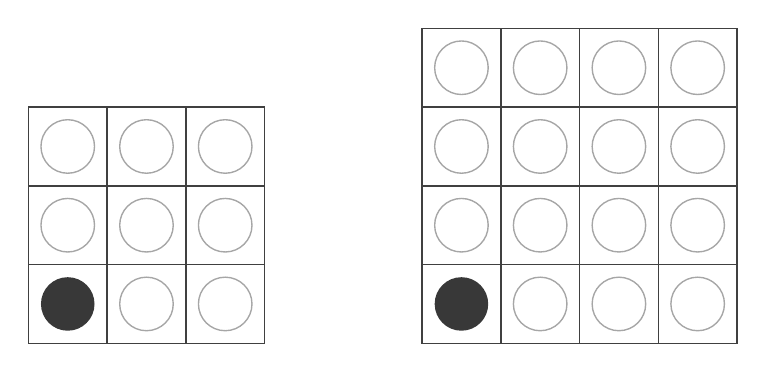
\begin{tikzpicture}[x=1mm, y=1mm]
\draw[line width=0.5pt, black!75] (0,0) rectangle ++(10,10);
\fill[black!78] (5,5) circle (3.4);
\draw[line width=0.5pt, black!75] (10,0) rectangle ++(10,10);
\draw[line width=0.5pt, black!35] (15,5) circle (3.4);
\draw[line width=0.5pt, black!75] (20,0) rectangle ++(10,10);
\draw[line width=0.5pt, black!35] (25,5) circle (3.4);
\draw[line width=0.5pt, black!75] (0,10) rectangle ++(10,10);
\draw[line width=0.5pt, black!35] (5,15) circle (3.4);
\draw[line width=0.5pt, black!75] (10,10) rectangle ++(10,10);
\draw[line width=0.5pt, black!35] (15,15) circle (3.4);
\draw[line width=0.5pt, black!75] (20,10) rectangle ++(10,10);
\draw[line width=0.5pt, black!35] (25,15) circle (3.4);
\draw[line width=0.5pt, black!75] (0,20) rectangle ++(10,10);
\draw[line width=0.5pt, black!35] (5,25) circle (3.4);
\draw[line width=0.5pt, black!75] (10,20) rectangle ++(10,10);
\draw[line width=0.5pt, black!35] (15,25) circle (3.4);
\draw[line width=0.5pt, black!75] (20,20) rectangle ++(10,10);
\draw[line width=0.5pt, black!35] (25,25) circle (3.4);
\draw[line width=0.5pt, black!75] (50,0) rectangle ++(10,10);
\fill[black!78] (55,5) circle (3.4);
\draw[line width=0.5pt, black!75] (60,0) rectangle ++(10,10);
\draw[line width=0.5pt, black!35] (65,5) circle (3.4);
\draw[line width=0.5pt, black!75] (70,0) rectangle ++(10,10);
\draw[line width=0.5pt, black!35] (75,5) circle (3.4);
\draw[line width=0.5pt, black!75] (80,0) rectangle ++(10,10);
\draw[line width=0.5pt, black!35] (85,5) circle (3.4);
\draw[line width=0.5pt, black!75] (50,10) rectangle ++(10,10);
\draw[line width=0.5pt, black!35] (55,15) circle (3.4);
\draw[line width=0.5pt, black!75] (60,10) rectangle ++(10,10);
\draw[line width=0.5pt, black!35] (65,15) circle (3.4);
\draw[line width=0.5pt, black!75] (70,10) rectangle ++(10,10);
\draw[line width=0.5pt, black!35] (75,15) circle (3.4);
\draw[line width=0.5pt, black!75] (80,10) rectangle ++(10,10);
\draw[line width=0.5pt, black!35] (85,15) circle (3.4);
\draw[line width=0.5pt, black!75] (50,20) rectangle ++(10,10);
\draw[line width=0.5pt, black!35] (55,25) circle (3.4);
\draw[line width=0.5pt, black!75] (60,20) rectangle ++(10,10);
\draw[line width=0.5pt, black!35] (65,25) circle (3.4);
\draw[line width=0.5pt, black!75] (70,20) rectangle ++(10,10);
\draw[line width=0.5pt, black!35] (75,25) circle (3.4);
\draw[line width=0.5pt, black!75] (80,20) rectangle ++(10,10);
\draw[line width=0.5pt, black!35] (85,25) circle (3.4);
\draw[line width=0.5pt, black!75] (50,30) rectangle ++(10,10);
\draw[line width=0.5pt, black!35] (55,35) circle (3.4);
\draw[line width=0.5pt, black!75] (60,30) rectangle ++(10,10);
\draw[line width=0.5pt, black!35] (65,35) circle (3.4);
\draw[line width=0.5pt, black!75] (70,30) rectangle ++(10,10);
\draw[line width=0.5pt, black!35] (75,35) circle (3.4);
\draw[line width=0.5pt, black!75] (80,30) rectangle ++(10,10);
\draw[line width=0.5pt, black!35] (85,35) circle (3.4);
\end{tikzpicture}\par\vspace{0mm}
\newpage
\prob{2}For each board below, decide whether the player whose turn it is can make sure to win. Write W in its box if so, and L if not.\par\vspace{6mm}
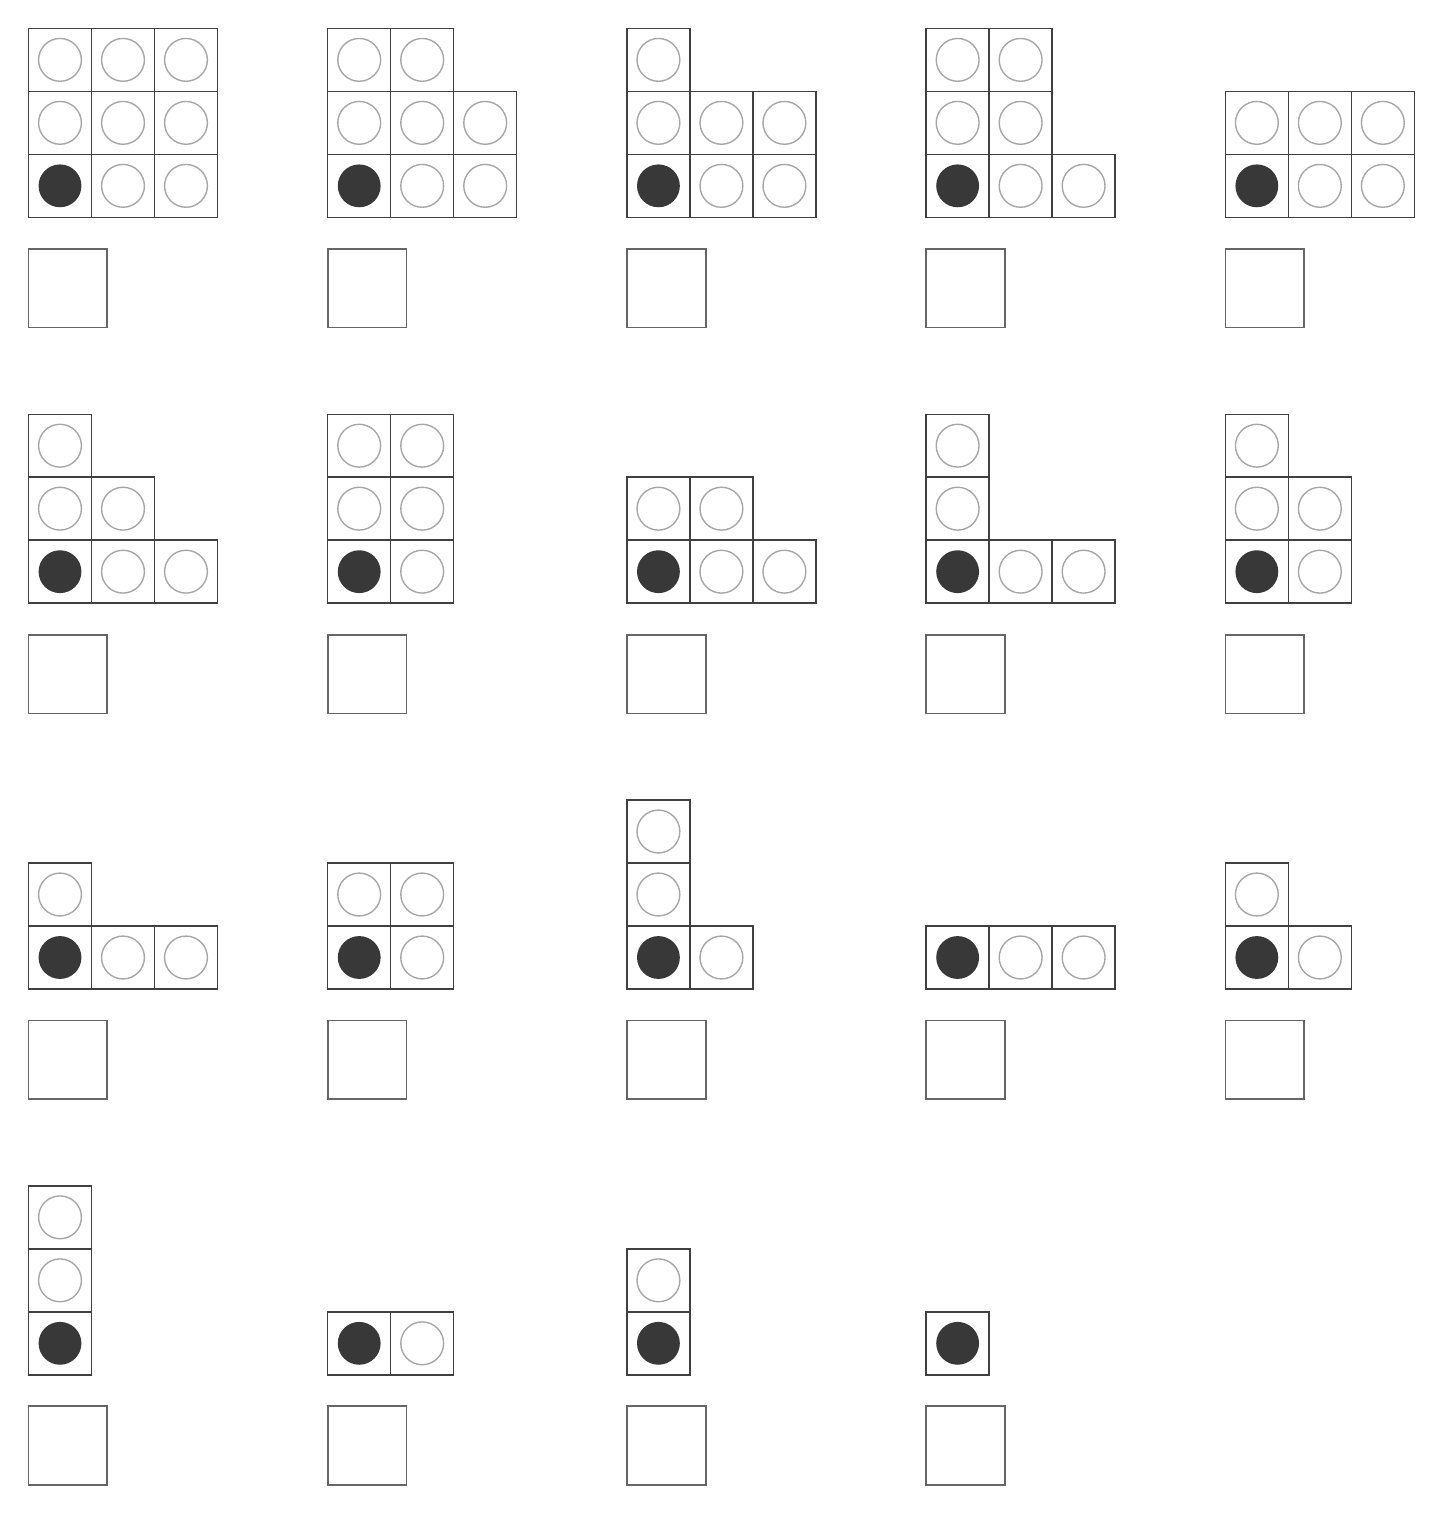
\begin{tikzpicture}[x=1mm, y=1mm]
\draw[line width=0.5pt, black!75] (0,-24) rectangle ++(8,8);
\fill[black!78] (4,-20) circle (2.72);
\draw[line width=0.5pt, black!75] (8,-24) rectangle ++(8,8);
\draw[line width=0.5pt, black!35] (12,-20) circle (2.72);
\draw[line width=0.5pt, black!75] (16,-24) rectangle ++(8,8);
\draw[line width=0.5pt, black!35] (20,-20) circle (2.72);
\draw[line width=0.5pt, black!75] (0,-16) rectangle ++(8,8);
\draw[line width=0.5pt, black!35] (4,-12) circle (2.72);
\draw[line width=0.5pt, black!75] (8,-16) rectangle ++(8,8);
\draw[line width=0.5pt, black!35] (12,-12) circle (2.72);
\draw[line width=0.5pt, black!75] (16,-16) rectangle ++(8,8);
\draw[line width=0.5pt, black!35] (20,-12) circle (2.72);
\draw[line width=0.5pt, black!75] (0,-8) rectangle ++(8,8);
\draw[line width=0.5pt, black!35] (4,-4) circle (2.72);
\draw[line width=0.5pt, black!75] (8,-8) rectangle ++(8,8);
\draw[line width=0.5pt, black!35] (12,-4) circle (2.72);
\draw[line width=0.5pt, black!75] (16,-8) rectangle ++(8,8);
\draw[line width=0.5pt, black!35] (20,-4) circle (2.72);
\draw[line width=0.6pt, black!60] (0,-38) rectangle ++(10,10);
\draw[line width=0.5pt, black!75] (38,-24) rectangle ++(8,8);
\fill[black!78] (42,-20) circle (2.72);
\draw[line width=0.5pt, black!75] (46,-24) rectangle ++(8,8);
\draw[line width=0.5pt, black!35] (50,-20) circle (2.72);
\draw[line width=0.5pt, black!75] (54,-24) rectangle ++(8,8);
\draw[line width=0.5pt, black!35] (58,-20) circle (2.72);
\draw[line width=0.5pt, black!75] (38,-16) rectangle ++(8,8);
\draw[line width=0.5pt, black!35] (42,-12) circle (2.72);
\draw[line width=0.5pt, black!75] (46,-16) rectangle ++(8,8);
\draw[line width=0.5pt, black!35] (50,-12) circle (2.72);
\draw[line width=0.5pt, black!75] (54,-16) rectangle ++(8,8);
\draw[line width=0.5pt, black!35] (58,-12) circle (2.72);
\draw[line width=0.5pt, black!75] (38,-8) rectangle ++(8,8);
\draw[line width=0.5pt, black!35] (42,-4) circle (2.72);
\draw[line width=0.5pt, black!75] (46,-8) rectangle ++(8,8);
\draw[line width=0.5pt, black!35] (50,-4) circle (2.72);
\draw[line width=0.6pt, black!60] (38,-38) rectangle ++(10,10);
\draw[line width=0.5pt, black!75] (76,-24) rectangle ++(8,8);
\fill[black!78] (80,-20) circle (2.72);
\draw[line width=0.5pt, black!75] (84,-24) rectangle ++(8,8);
\draw[line width=0.5pt, black!35] (88,-20) circle (2.72);
\draw[line width=0.5pt, black!75] (92,-24) rectangle ++(8,8);
\draw[line width=0.5pt, black!35] (96,-20) circle (2.72);
\draw[line width=0.5pt, black!75] (76,-16) rectangle ++(8,8);
\draw[line width=0.5pt, black!35] (80,-12) circle (2.72);
\draw[line width=0.5pt, black!75] (84,-16) rectangle ++(8,8);
\draw[line width=0.5pt, black!35] (88,-12) circle (2.72);
\draw[line width=0.5pt, black!75] (92,-16) rectangle ++(8,8);
\draw[line width=0.5pt, black!35] (96,-12) circle (2.72);
\draw[line width=0.5pt, black!75] (76,-8) rectangle ++(8,8);
\draw[line width=0.5pt, black!35] (80,-4) circle (2.72);
\draw[line width=0.6pt, black!60] (76,-38) rectangle ++(10,10);
\draw[line width=0.5pt, black!75] (114,-24) rectangle ++(8,8);
\fill[black!78] (118,-20) circle (2.72);
\draw[line width=0.5pt, black!75] (122,-24) rectangle ++(8,8);
\draw[line width=0.5pt, black!35] (126,-20) circle (2.72);
\draw[line width=0.5pt, black!75] (130,-24) rectangle ++(8,8);
\draw[line width=0.5pt, black!35] (134,-20) circle (2.72);
\draw[line width=0.5pt, black!75] (114,-16) rectangle ++(8,8);
\draw[line width=0.5pt, black!35] (118,-12) circle (2.72);
\draw[line width=0.5pt, black!75] (122,-16) rectangle ++(8,8);
\draw[line width=0.5pt, black!35] (126,-12) circle (2.72);
\draw[line width=0.5pt, black!75] (114,-8) rectangle ++(8,8);
\draw[line width=0.5pt, black!35] (118,-4) circle (2.72);
\draw[line width=0.5pt, black!75] (122,-8) rectangle ++(8,8);
\draw[line width=0.5pt, black!35] (126,-4) circle (2.72);
\draw[line width=0.6pt, black!60] (114,-38) rectangle ++(10,10);
\draw[line width=0.5pt, black!75] (152,-24) rectangle ++(8,8);
\fill[black!78] (156,-20) circle (2.72);
\draw[line width=0.5pt, black!75] (160,-24) rectangle ++(8,8);
\draw[line width=0.5pt, black!35] (164,-20) circle (2.72);
\draw[line width=0.5pt, black!75] (168,-24) rectangle ++(8,8);
\draw[line width=0.5pt, black!35] (172,-20) circle (2.72);
\draw[line width=0.5pt, black!75] (152,-16) rectangle ++(8,8);
\draw[line width=0.5pt, black!35] (156,-12) circle (2.72);
\draw[line width=0.5pt, black!75] (160,-16) rectangle ++(8,8);
\draw[line width=0.5pt, black!35] (164,-12) circle (2.72);
\draw[line width=0.5pt, black!75] (168,-16) rectangle ++(8,8);
\draw[line width=0.5pt, black!35] (172,-12) circle (2.72);
\draw[line width=0.6pt, black!60] (152,-38) rectangle ++(10,10);
\draw[line width=0.5pt, black!75] (0,-73) rectangle ++(8,8);
\fill[black!78] (4,-69) circle (2.72);
\draw[line width=0.5pt, black!75] (8,-73) rectangle ++(8,8);
\draw[line width=0.5pt, black!35] (12,-69) circle (2.72);
\draw[line width=0.5pt, black!75] (16,-73) rectangle ++(8,8);
\draw[line width=0.5pt, black!35] (20,-69) circle (2.72);
\draw[line width=0.5pt, black!75] (0,-65) rectangle ++(8,8);
\draw[line width=0.5pt, black!35] (4,-61) circle (2.72);
\draw[line width=0.5pt, black!75] (8,-65) rectangle ++(8,8);
\draw[line width=0.5pt, black!35] (12,-61) circle (2.72);
\draw[line width=0.5pt, black!75] (0,-57) rectangle ++(8,8);
\draw[line width=0.5pt, black!35] (4,-53) circle (2.72);
\draw[line width=0.6pt, black!60] (0,-87) rectangle ++(10,10);
\draw[line width=0.5pt, black!75] (38,-73) rectangle ++(8,8);
\fill[black!78] (42,-69) circle (2.72);
\draw[line width=0.5pt, black!75] (46,-73) rectangle ++(8,8);
\draw[line width=0.5pt, black!35] (50,-69) circle (2.72);
\draw[line width=0.5pt, black!75] (38,-65) rectangle ++(8,8);
\draw[line width=0.5pt, black!35] (42,-61) circle (2.72);
\draw[line width=0.5pt, black!75] (46,-65) rectangle ++(8,8);
\draw[line width=0.5pt, black!35] (50,-61) circle (2.72);
\draw[line width=0.5pt, black!75] (38,-57) rectangle ++(8,8);
\draw[line width=0.5pt, black!35] (42,-53) circle (2.72);
\draw[line width=0.5pt, black!75] (46,-57) rectangle ++(8,8);
\draw[line width=0.5pt, black!35] (50,-53) circle (2.72);
\draw[line width=0.6pt, black!60] (38,-87) rectangle ++(10,10);
\draw[line width=0.5pt, black!75] (76,-73) rectangle ++(8,8);
\fill[black!78] (80,-69) circle (2.72);
\draw[line width=0.5pt, black!75] (84,-73) rectangle ++(8,8);
\draw[line width=0.5pt, black!35] (88,-69) circle (2.72);
\draw[line width=0.5pt, black!75] (92,-73) rectangle ++(8,8);
\draw[line width=0.5pt, black!35] (96,-69) circle (2.72);
\draw[line width=0.5pt, black!75] (76,-65) rectangle ++(8,8);
\draw[line width=0.5pt, black!35] (80,-61) circle (2.72);
\draw[line width=0.5pt, black!75] (84,-65) rectangle ++(8,8);
\draw[line width=0.5pt, black!35] (88,-61) circle (2.72);
\draw[line width=0.6pt, black!60] (76,-87) rectangle ++(10,10);
\draw[line width=0.5pt, black!75] (114,-73) rectangle ++(8,8);
\fill[black!78] (118,-69) circle (2.72);
\draw[line width=0.5pt, black!75] (122,-73) rectangle ++(8,8);
\draw[line width=0.5pt, black!35] (126,-69) circle (2.72);
\draw[line width=0.5pt, black!75] (130,-73) rectangle ++(8,8);
\draw[line width=0.5pt, black!35] (134,-69) circle (2.72);
\draw[line width=0.5pt, black!75] (114,-65) rectangle ++(8,8);
\draw[line width=0.5pt, black!35] (118,-61) circle (2.72);
\draw[line width=0.5pt, black!75] (114,-57) rectangle ++(8,8);
\draw[line width=0.5pt, black!35] (118,-53) circle (2.72);
\draw[line width=0.6pt, black!60] (114,-87) rectangle ++(10,10);
\draw[line width=0.5pt, black!75] (152,-73) rectangle ++(8,8);
\fill[black!78] (156,-69) circle (2.72);
\draw[line width=0.5pt, black!75] (160,-73) rectangle ++(8,8);
\draw[line width=0.5pt, black!35] (164,-69) circle (2.72);
\draw[line width=0.5pt, black!75] (152,-65) rectangle ++(8,8);
\draw[line width=0.5pt, black!35] (156,-61) circle (2.72);
\draw[line width=0.5pt, black!75] (160,-65) rectangle ++(8,8);
\draw[line width=0.5pt, black!35] (164,-61) circle (2.72);
\draw[line width=0.5pt, black!75] (152,-57) rectangle ++(8,8);
\draw[line width=0.5pt, black!35] (156,-53) circle (2.72);
\draw[line width=0.6pt, black!60] (152,-87) rectangle ++(10,10);
\draw[line width=0.5pt, black!75] (0,-122) rectangle ++(8,8);
\fill[black!78] (4,-118) circle (2.72);
\draw[line width=0.5pt, black!75] (8,-122) rectangle ++(8,8);
\draw[line width=0.5pt, black!35] (12,-118) circle (2.72);
\draw[line width=0.5pt, black!75] (16,-122) rectangle ++(8,8);
\draw[line width=0.5pt, black!35] (20,-118) circle (2.72);
\draw[line width=0.5pt, black!75] (0,-114) rectangle ++(8,8);
\draw[line width=0.5pt, black!35] (4,-110) circle (2.72);
\draw[line width=0.6pt, black!60] (0,-136) rectangle ++(10,10);
\draw[line width=0.5pt, black!75] (38,-122) rectangle ++(8,8);
\fill[black!78] (42,-118) circle (2.72);
\draw[line width=0.5pt, black!75] (46,-122) rectangle ++(8,8);
\draw[line width=0.5pt, black!35] (50,-118) circle (2.72);
\draw[line width=0.5pt, black!75] (38,-114) rectangle ++(8,8);
\draw[line width=0.5pt, black!35] (42,-110) circle (2.72);
\draw[line width=0.5pt, black!75] (46,-114) rectangle ++(8,8);
\draw[line width=0.5pt, black!35] (50,-110) circle (2.72);
\draw[line width=0.6pt, black!60] (38,-136) rectangle ++(10,10);
\draw[line width=0.5pt, black!75] (76,-122) rectangle ++(8,8);
\fill[black!78] (80,-118) circle (2.72);
\draw[line width=0.5pt, black!75] (84,-122) rectangle ++(8,8);
\draw[line width=0.5pt, black!35] (88,-118) circle (2.72);
\draw[line width=0.5pt, black!75] (76,-114) rectangle ++(8,8);
\draw[line width=0.5pt, black!35] (80,-110) circle (2.72);
\draw[line width=0.5pt, black!75] (76,-106) rectangle ++(8,8);
\draw[line width=0.5pt, black!35] (80,-102) circle (2.72);
\draw[line width=0.6pt, black!60] (76,-136) rectangle ++(10,10);
\draw[line width=0.5pt, black!75] (114,-122) rectangle ++(8,8);
\fill[black!78] (118,-118) circle (2.72);
\draw[line width=0.5pt, black!75] (122,-122) rectangle ++(8,8);
\draw[line width=0.5pt, black!35] (126,-118) circle (2.72);
\draw[line width=0.5pt, black!75] (130,-122) rectangle ++(8,8);
\draw[line width=0.5pt, black!35] (134,-118) circle (2.72);
\draw[line width=0.6pt, black!60] (114,-136) rectangle ++(10,10);
\draw[line width=0.5pt, black!75] (152,-122) rectangle ++(8,8);
\fill[black!78] (156,-118) circle (2.72);
\draw[line width=0.5pt, black!75] (160,-122) rectangle ++(8,8);
\draw[line width=0.5pt, black!35] (164,-118) circle (2.72);
\draw[line width=0.5pt, black!75] (152,-114) rectangle ++(8,8);
\draw[line width=0.5pt, black!35] (156,-110) circle (2.72);
\draw[line width=0.6pt, black!60] (152,-136) rectangle ++(10,10);
\draw[line width=0.5pt, black!75] (0,-171) rectangle ++(8,8);
\fill[black!78] (4,-167) circle (2.72);
\draw[line width=0.5pt, black!75] (0,-163) rectangle ++(8,8);
\draw[line width=0.5pt, black!35] (4,-159) circle (2.72);
\draw[line width=0.5pt, black!75] (0,-155) rectangle ++(8,8);
\draw[line width=0.5pt, black!35] (4,-151) circle (2.72);
\draw[line width=0.6pt, black!60] (0,-185) rectangle ++(10,10);
\draw[line width=0.5pt, black!75] (38,-171) rectangle ++(8,8);
\fill[black!78] (42,-167) circle (2.72);
\draw[line width=0.5pt, black!75] (46,-171) rectangle ++(8,8);
\draw[line width=0.5pt, black!35] (50,-167) circle (2.72);
\draw[line width=0.6pt, black!60] (38,-185) rectangle ++(10,10);
\draw[line width=0.5pt, black!75] (76,-171) rectangle ++(8,8);
\fill[black!78] (80,-167) circle (2.72);
\draw[line width=0.5pt, black!75] (76,-163) rectangle ++(8,8);
\draw[line width=0.5pt, black!35] (80,-159) circle (2.72);
\draw[line width=0.6pt, black!60] (76,-185) rectangle ++(10,10);
\draw[line width=0.5pt, black!75] (114,-171) rectangle ++(8,8);
\fill[black!78] (118,-167) circle (2.72);
\draw[line width=0.6pt, black!60] (114,-185) rectangle ++(10,10);
\end{tikzpicture}\par\vspace{0mm}
\newpage
\prob{3}It is your turn on each board. If you can make sure to win, mark your first bite.\par\vspace{5mm}
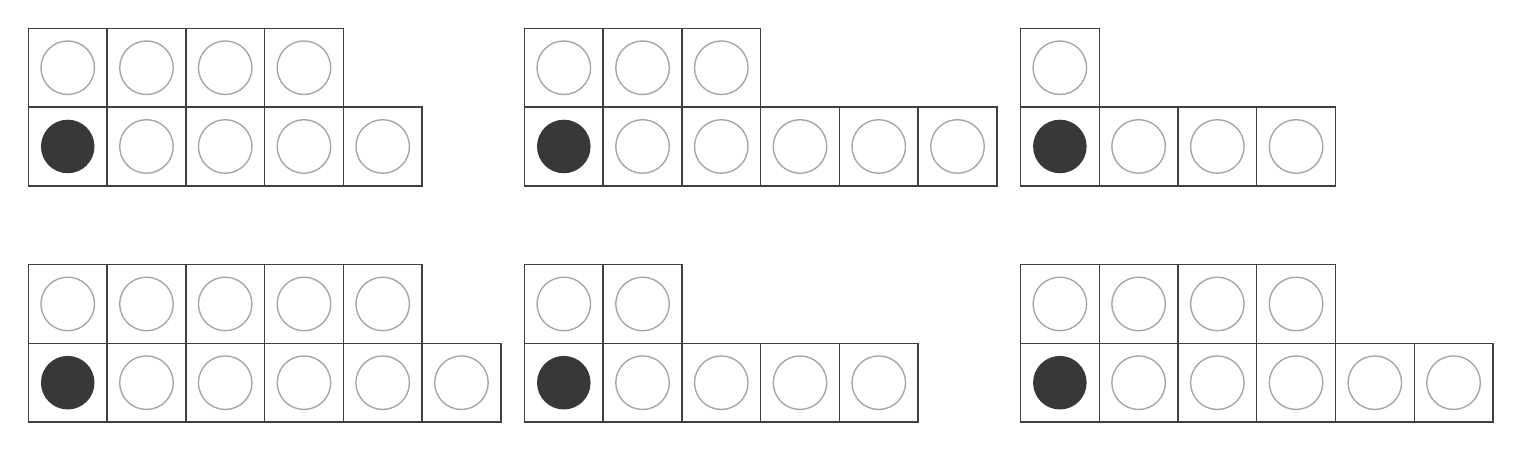
\begin{tikzpicture}[x=1mm, y=1mm]
\draw[line width=0.5pt, black!75] (0,-20) rectangle ++(10,10);
\fill[black!78] (5,-15) circle (3.4);
\draw[line width=0.5pt, black!75] (10,-20) rectangle ++(10,10);
\draw[line width=0.5pt, black!35] (15,-15) circle (3.4);
\draw[line width=0.5pt, black!75] (20,-20) rectangle ++(10,10);
\draw[line width=0.5pt, black!35] (25,-15) circle (3.4);
\draw[line width=0.5pt, black!75] (30,-20) rectangle ++(10,10);
\draw[line width=0.5pt, black!35] (35,-15) circle (3.4);
\draw[line width=0.5pt, black!75] (40,-20) rectangle ++(10,10);
\draw[line width=0.5pt, black!35] (45,-15) circle (3.4);
\draw[line width=0.5pt, black!75] (0,-10) rectangle ++(10,10);
\draw[line width=0.5pt, black!35] (5,-5) circle (3.4);
\draw[line width=0.5pt, black!75] (10,-10) rectangle ++(10,10);
\draw[line width=0.5pt, black!35] (15,-5) circle (3.4);
\draw[line width=0.5pt, black!75] (20,-10) rectangle ++(10,10);
\draw[line width=0.5pt, black!35] (25,-5) circle (3.4);
\draw[line width=0.5pt, black!75] (30,-10) rectangle ++(10,10);
\draw[line width=0.5pt, black!35] (35,-5) circle (3.4);
\draw[line width=0.5pt, black!75] (63,-20) rectangle ++(10,10);
\fill[black!78] (68,-15) circle (3.4);
\draw[line width=0.5pt, black!75] (73,-20) rectangle ++(10,10);
\draw[line width=0.5pt, black!35] (78,-15) circle (3.4);
\draw[line width=0.5pt, black!75] (83,-20) rectangle ++(10,10);
\draw[line width=0.5pt, black!35] (88,-15) circle (3.4);
\draw[line width=0.5pt, black!75] (93,-20) rectangle ++(10,10);
\draw[line width=0.5pt, black!35] (98,-15) circle (3.4);
\draw[line width=0.5pt, black!75] (103,-20) rectangle ++(10,10);
\draw[line width=0.5pt, black!35] (108,-15) circle (3.4);
\draw[line width=0.5pt, black!75] (113,-20) rectangle ++(10,10);
\draw[line width=0.5pt, black!35] (118,-15) circle (3.4);
\draw[line width=0.5pt, black!75] (63,-10) rectangle ++(10,10);
\draw[line width=0.5pt, black!35] (68,-5) circle (3.4);
\draw[line width=0.5pt, black!75] (73,-10) rectangle ++(10,10);
\draw[line width=0.5pt, black!35] (78,-5) circle (3.4);
\draw[line width=0.5pt, black!75] (83,-10) rectangle ++(10,10);
\draw[line width=0.5pt, black!35] (88,-5) circle (3.4);
\draw[line width=0.5pt, black!75] (126,-20) rectangle ++(10,10);
\fill[black!78] (131,-15) circle (3.4);
\draw[line width=0.5pt, black!75] (136,-20) rectangle ++(10,10);
\draw[line width=0.5pt, black!35] (141,-15) circle (3.4);
\draw[line width=0.5pt, black!75] (146,-20) rectangle ++(10,10);
\draw[line width=0.5pt, black!35] (151,-15) circle (3.4);
\draw[line width=0.5pt, black!75] (156,-20) rectangle ++(10,10);
\draw[line width=0.5pt, black!35] (161,-15) circle (3.4);
\draw[line width=0.5pt, black!75] (126,-10) rectangle ++(10,10);
\draw[line width=0.5pt, black!35] (131,-5) circle (3.4);
\draw[line width=0.5pt, black!75] (0,-50) rectangle ++(10,10);
\fill[black!78] (5,-45) circle (3.4);
\draw[line width=0.5pt, black!75] (10,-50) rectangle ++(10,10);
\draw[line width=0.5pt, black!35] (15,-45) circle (3.4);
\draw[line width=0.5pt, black!75] (20,-50) rectangle ++(10,10);
\draw[line width=0.5pt, black!35] (25,-45) circle (3.4);
\draw[line width=0.5pt, black!75] (30,-50) rectangle ++(10,10);
\draw[line width=0.5pt, black!35] (35,-45) circle (3.4);
\draw[line width=0.5pt, black!75] (40,-50) rectangle ++(10,10);
\draw[line width=0.5pt, black!35] (45,-45) circle (3.4);
\draw[line width=0.5pt, black!75] (50,-50) rectangle ++(10,10);
\draw[line width=0.5pt, black!35] (55,-45) circle (3.4);
\draw[line width=0.5pt, black!75] (0,-40) rectangle ++(10,10);
\draw[line width=0.5pt, black!35] (5,-35) circle (3.4);
\draw[line width=0.5pt, black!75] (10,-40) rectangle ++(10,10);
\draw[line width=0.5pt, black!35] (15,-35) circle (3.4);
\draw[line width=0.5pt, black!75] (20,-40) rectangle ++(10,10);
\draw[line width=0.5pt, black!35] (25,-35) circle (3.4);
\draw[line width=0.5pt, black!75] (30,-40) rectangle ++(10,10);
\draw[line width=0.5pt, black!35] (35,-35) circle (3.4);
\draw[line width=0.5pt, black!75] (40,-40) rectangle ++(10,10);
\draw[line width=0.5pt, black!35] (45,-35) circle (3.4);
\draw[line width=0.5pt, black!75] (63,-50) rectangle ++(10,10);
\fill[black!78] (68,-45) circle (3.4);
\draw[line width=0.5pt, black!75] (73,-50) rectangle ++(10,10);
\draw[line width=0.5pt, black!35] (78,-45) circle (3.4);
\draw[line width=0.5pt, black!75] (83,-50) rectangle ++(10,10);
\draw[line width=0.5pt, black!35] (88,-45) circle (3.4);
\draw[line width=0.5pt, black!75] (93,-50) rectangle ++(10,10);
\draw[line width=0.5pt, black!35] (98,-45) circle (3.4);
\draw[line width=0.5pt, black!75] (103,-50) rectangle ++(10,10);
\draw[line width=0.5pt, black!35] (108,-45) circle (3.4);
\draw[line width=0.5pt, black!75] (63,-40) rectangle ++(10,10);
\draw[line width=0.5pt, black!35] (68,-35) circle (3.4);
\draw[line width=0.5pt, black!75] (73,-40) rectangle ++(10,10);
\draw[line width=0.5pt, black!35] (78,-35) circle (3.4);
\draw[line width=0.5pt, black!75] (126,-50) rectangle ++(10,10);
\fill[black!78] (131,-45) circle (3.4);
\draw[line width=0.5pt, black!75] (136,-50) rectangle ++(10,10);
\draw[line width=0.5pt, black!35] (141,-45) circle (3.4);
\draw[line width=0.5pt, black!75] (146,-50) rectangle ++(10,10);
\draw[line width=0.5pt, black!35] (151,-45) circle (3.4);
\draw[line width=0.5pt, black!75] (156,-50) rectangle ++(10,10);
\draw[line width=0.5pt, black!35] (161,-45) circle (3.4);
\draw[line width=0.5pt, black!75] (166,-50) rectangle ++(10,10);
\draw[line width=0.5pt, black!35] (171,-45) circle (3.4);
\draw[line width=0.5pt, black!75] (176,-50) rectangle ++(10,10);
\draw[line width=0.5pt, black!35] (181,-45) circle (3.4);
\draw[line width=0.5pt, black!75] (126,-40) rectangle ++(10,10);
\draw[line width=0.5pt, black!35] (131,-35) circle (3.4);
\draw[line width=0.5pt, black!75] (136,-40) rectangle ++(10,10);
\draw[line width=0.5pt, black!35] (141,-35) circle (3.4);
\draw[line width=0.5pt, black!75] (146,-40) rectangle ++(10,10);
\draw[line width=0.5pt, black!35] (151,-35) circle (3.4);
\draw[line width=0.5pt, black!75] (156,-40) rectangle ++(10,10);
\draw[line width=0.5pt, black!35] (161,-35) circle (3.4);
\end{tikzpicture}\par\vspace{12mm}
\prob{4}Explain how the first player can make sure to win on every rectangle with two rows and on every square bigger than one cookie, however long the sides are.\par\vspace{0mm}
\newpage
\prob{5}Mark every first bite on the 3 by 4 board after which the first player can make sure to win.\par\vspace{5mm}
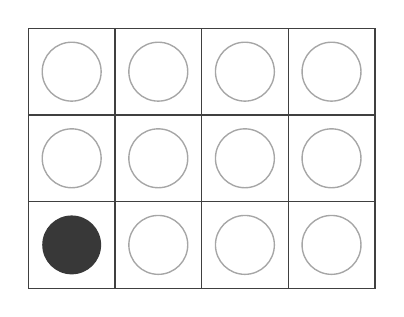
\begin{tikzpicture}[x=1mm, y=1mm]
\draw[line width=0.5pt, black!75] (0,0) rectangle ++(11,11);
\fill[black!78] (5.5,5.5) circle (3.74);
\draw[line width=0.5pt, black!75] (11,0) rectangle ++(11,11);
\draw[line width=0.5pt, black!35] (16.5,5.5) circle (3.74);
\draw[line width=0.5pt, black!75] (22,0) rectangle ++(11,11);
\draw[line width=0.5pt, black!35] (27.5,5.5) circle (3.74);
\draw[line width=0.5pt, black!75] (33,0) rectangle ++(11,11);
\draw[line width=0.5pt, black!35] (38.5,5.5) circle (3.74);
\draw[line width=0.5pt, black!75] (0,11) rectangle ++(11,11);
\draw[line width=0.5pt, black!35] (5.5,16.5) circle (3.74);
\draw[line width=0.5pt, black!75] (11,11) rectangle ++(11,11);
\draw[line width=0.5pt, black!35] (16.5,16.5) circle (3.74);
\draw[line width=0.5pt, black!75] (22,11) rectangle ++(11,11);
\draw[line width=0.5pt, black!35] (27.5,16.5) circle (3.74);
\draw[line width=0.5pt, black!75] (33,11) rectangle ++(11,11);
\draw[line width=0.5pt, black!35] (38.5,16.5) circle (3.74);
\draw[line width=0.5pt, black!75] (0,22) rectangle ++(11,11);
\draw[line width=0.5pt, black!35] (5.5,27.5) circle (3.74);
\draw[line width=0.5pt, black!75] (11,22) rectangle ++(11,11);
\draw[line width=0.5pt, black!35] (16.5,27.5) circle (3.74);
\draw[line width=0.5pt, black!75] (22,22) rectangle ++(11,11);
\draw[line width=0.5pt, black!35] (27.5,27.5) circle (3.74);
\draw[line width=0.5pt, black!75] (33,22) rectangle ++(11,11);
\draw[line width=0.5pt, black!35] (38.5,27.5) circle (3.74);
\end{tikzpicture}\par\vspace{12mm}
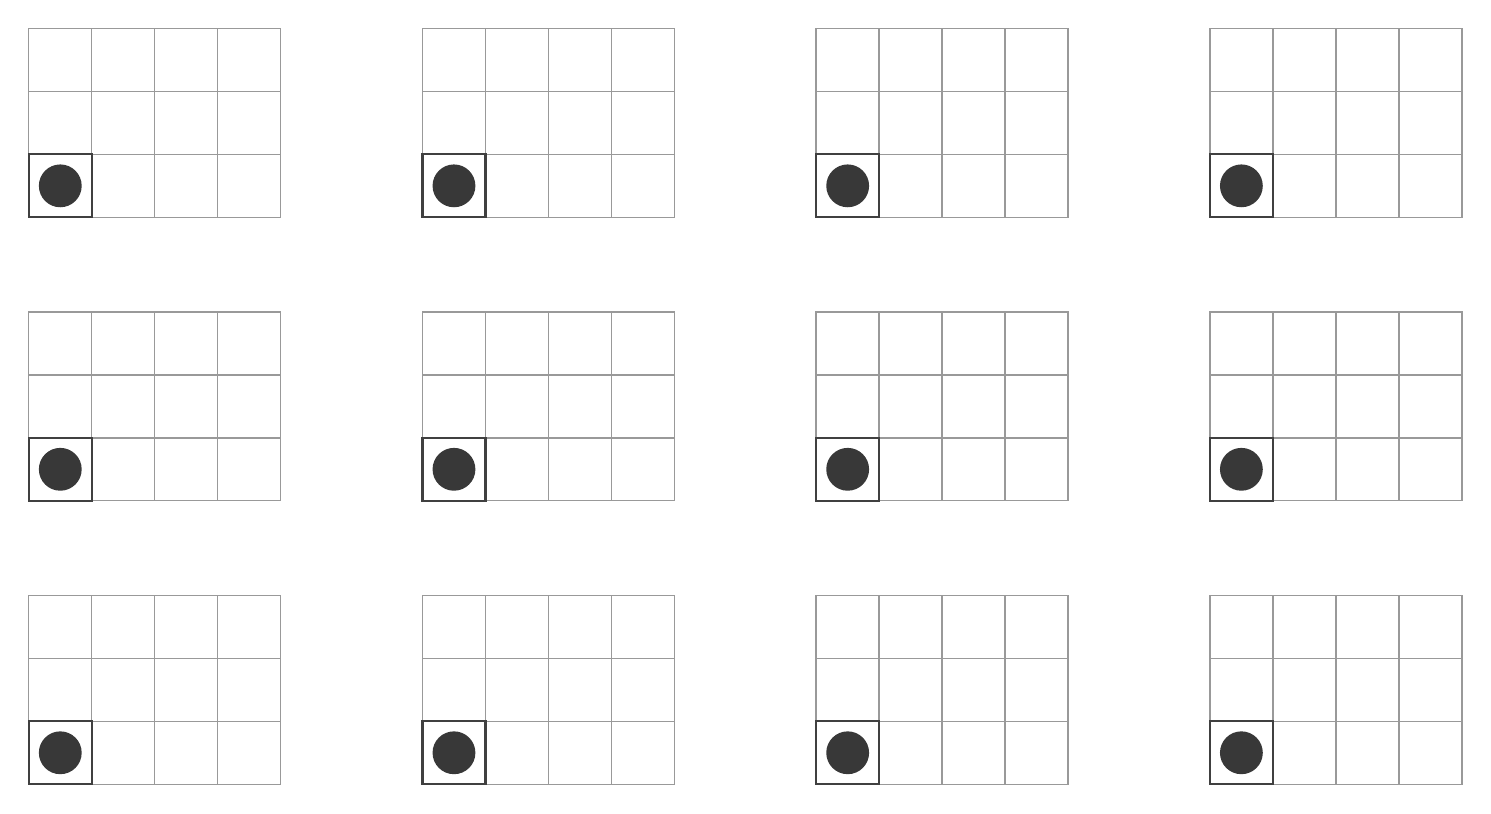
\begin{tikzpicture}[x=1mm, y=1mm]
\draw[line width=0.5pt, black!40] (0,0) rectangle ++(8,8);
\draw[line width=0.5pt, black!40] (8,0) rectangle ++(8,8);
\draw[line width=0.5pt, black!40] (16,0) rectangle ++(8,8);
\draw[line width=0.5pt, black!40] (24,0) rectangle ++(8,8);
\draw[line width=0.5pt, black!40] (0,8) rectangle ++(8,8);
\draw[line width=0.5pt, black!40] (8,8) rectangle ++(8,8);
\draw[line width=0.5pt, black!40] (16,8) rectangle ++(8,8);
\draw[line width=0.5pt, black!40] (24,8) rectangle ++(8,8);
\draw[line width=0.5pt, black!40] (0,16) rectangle ++(8,8);
\draw[line width=0.5pt, black!40] (8,16) rectangle ++(8,8);
\draw[line width=0.5pt, black!40] (16,16) rectangle ++(8,8);
\draw[line width=0.5pt, black!40] (24,16) rectangle ++(8,8);
\fill[black!78] (4,4) circle (2.72);
\draw[line width=0.8pt, black!75] (0,0) rectangle ++(8,8);
\draw[line width=0.5pt, black!40] (50,0) rectangle ++(8,8);
\draw[line width=0.5pt, black!40] (58,0) rectangle ++(8,8);
\draw[line width=0.5pt, black!40] (66,0) rectangle ++(8,8);
\draw[line width=0.5pt, black!40] (74,0) rectangle ++(8,8);
\draw[line width=0.5pt, black!40] (50,8) rectangle ++(8,8);
\draw[line width=0.5pt, black!40] (58,8) rectangle ++(8,8);
\draw[line width=0.5pt, black!40] (66,8) rectangle ++(8,8);
\draw[line width=0.5pt, black!40] (74,8) rectangle ++(8,8);
\draw[line width=0.5pt, black!40] (50,16) rectangle ++(8,8);
\draw[line width=0.5pt, black!40] (58,16) rectangle ++(8,8);
\draw[line width=0.5pt, black!40] (66,16) rectangle ++(8,8);
\draw[line width=0.5pt, black!40] (74,16) rectangle ++(8,8);
\fill[black!78] (54,4) circle (2.72);
\draw[line width=0.8pt, black!75] (50,0) rectangle ++(8,8);
\draw[line width=0.5pt, black!40] (100,0) rectangle ++(8,8);
\draw[line width=0.5pt, black!40] (108,0) rectangle ++(8,8);
\draw[line width=0.5pt, black!40] (116,0) rectangle ++(8,8);
\draw[line width=0.5pt, black!40] (124,0) rectangle ++(8,8);
\draw[line width=0.5pt, black!40] (100,8) rectangle ++(8,8);
\draw[line width=0.5pt, black!40] (108,8) rectangle ++(8,8);
\draw[line width=0.5pt, black!40] (116,8) rectangle ++(8,8);
\draw[line width=0.5pt, black!40] (124,8) rectangle ++(8,8);
\draw[line width=0.5pt, black!40] (100,16) rectangle ++(8,8);
\draw[line width=0.5pt, black!40] (108,16) rectangle ++(8,8);
\draw[line width=0.5pt, black!40] (116,16) rectangle ++(8,8);
\draw[line width=0.5pt, black!40] (124,16) rectangle ++(8,8);
\fill[black!78] (104,4) circle (2.72);
\draw[line width=0.8pt, black!75] (100,0) rectangle ++(8,8);
\draw[line width=0.5pt, black!40] (150,0) rectangle ++(8,8);
\draw[line width=0.5pt, black!40] (158,0) rectangle ++(8,8);
\draw[line width=0.5pt, black!40] (166,0) rectangle ++(8,8);
\draw[line width=0.5pt, black!40] (174,0) rectangle ++(8,8);
\draw[line width=0.5pt, black!40] (150,8) rectangle ++(8,8);
\draw[line width=0.5pt, black!40] (158,8) rectangle ++(8,8);
\draw[line width=0.5pt, black!40] (166,8) rectangle ++(8,8);
\draw[line width=0.5pt, black!40] (174,8) rectangle ++(8,8);
\draw[line width=0.5pt, black!40] (150,16) rectangle ++(8,8);
\draw[line width=0.5pt, black!40] (158,16) rectangle ++(8,8);
\draw[line width=0.5pt, black!40] (166,16) rectangle ++(8,8);
\draw[line width=0.5pt, black!40] (174,16) rectangle ++(8,8);
\fill[black!78] (154,4) circle (2.72);
\draw[line width=0.8pt, black!75] (150,0) rectangle ++(8,8);
\draw[line width=0.5pt, black!40] (0,-36) rectangle ++(8,8);
\draw[line width=0.5pt, black!40] (8,-36) rectangle ++(8,8);
\draw[line width=0.5pt, black!40] (16,-36) rectangle ++(8,8);
\draw[line width=0.5pt, black!40] (24,-36) rectangle ++(8,8);
\draw[line width=0.5pt, black!40] (0,-28) rectangle ++(8,8);
\draw[line width=0.5pt, black!40] (8,-28) rectangle ++(8,8);
\draw[line width=0.5pt, black!40] (16,-28) rectangle ++(8,8);
\draw[line width=0.5pt, black!40] (24,-28) rectangle ++(8,8);
\draw[line width=0.5pt, black!40] (0,-20) rectangle ++(8,8);
\draw[line width=0.5pt, black!40] (8,-20) rectangle ++(8,8);
\draw[line width=0.5pt, black!40] (16,-20) rectangle ++(8,8);
\draw[line width=0.5pt, black!40] (24,-20) rectangle ++(8,8);
\fill[black!78] (4,-32) circle (2.72);
\draw[line width=0.8pt, black!75] (0,-36) rectangle ++(8,8);
\draw[line width=0.5pt, black!40] (50,-36) rectangle ++(8,8);
\draw[line width=0.5pt, black!40] (58,-36) rectangle ++(8,8);
\draw[line width=0.5pt, black!40] (66,-36) rectangle ++(8,8);
\draw[line width=0.5pt, black!40] (74,-36) rectangle ++(8,8);
\draw[line width=0.5pt, black!40] (50,-28) rectangle ++(8,8);
\draw[line width=0.5pt, black!40] (58,-28) rectangle ++(8,8);
\draw[line width=0.5pt, black!40] (66,-28) rectangle ++(8,8);
\draw[line width=0.5pt, black!40] (74,-28) rectangle ++(8,8);
\draw[line width=0.5pt, black!40] (50,-20) rectangle ++(8,8);
\draw[line width=0.5pt, black!40] (58,-20) rectangle ++(8,8);
\draw[line width=0.5pt, black!40] (66,-20) rectangle ++(8,8);
\draw[line width=0.5pt, black!40] (74,-20) rectangle ++(8,8);
\fill[black!78] (54,-32) circle (2.72);
\draw[line width=0.8pt, black!75] (50,-36) rectangle ++(8,8);
\draw[line width=0.5pt, black!40] (100,-36) rectangle ++(8,8);
\draw[line width=0.5pt, black!40] (108,-36) rectangle ++(8,8);
\draw[line width=0.5pt, black!40] (116,-36) rectangle ++(8,8);
\draw[line width=0.5pt, black!40] (124,-36) rectangle ++(8,8);
\draw[line width=0.5pt, black!40] (100,-28) rectangle ++(8,8);
\draw[line width=0.5pt, black!40] (108,-28) rectangle ++(8,8);
\draw[line width=0.5pt, black!40] (116,-28) rectangle ++(8,8);
\draw[line width=0.5pt, black!40] (124,-28) rectangle ++(8,8);
\draw[line width=0.5pt, black!40] (100,-20) rectangle ++(8,8);
\draw[line width=0.5pt, black!40] (108,-20) rectangle ++(8,8);
\draw[line width=0.5pt, black!40] (116,-20) rectangle ++(8,8);
\draw[line width=0.5pt, black!40] (124,-20) rectangle ++(8,8);
\fill[black!78] (104,-32) circle (2.72);
\draw[line width=0.8pt, black!75] (100,-36) rectangle ++(8,8);
\draw[line width=0.5pt, black!40] (150,-36) rectangle ++(8,8);
\draw[line width=0.5pt, black!40] (158,-36) rectangle ++(8,8);
\draw[line width=0.5pt, black!40] (166,-36) rectangle ++(8,8);
\draw[line width=0.5pt, black!40] (174,-36) rectangle ++(8,8);
\draw[line width=0.5pt, black!40] (150,-28) rectangle ++(8,8);
\draw[line width=0.5pt, black!40] (158,-28) rectangle ++(8,8);
\draw[line width=0.5pt, black!40] (166,-28) rectangle ++(8,8);
\draw[line width=0.5pt, black!40] (174,-28) rectangle ++(8,8);
\draw[line width=0.5pt, black!40] (150,-20) rectangle ++(8,8);
\draw[line width=0.5pt, black!40] (158,-20) rectangle ++(8,8);
\draw[line width=0.5pt, black!40] (166,-20) rectangle ++(8,8);
\draw[line width=0.5pt, black!40] (174,-20) rectangle ++(8,8);
\fill[black!78] (154,-32) circle (2.72);
\draw[line width=0.8pt, black!75] (150,-36) rectangle ++(8,8);
\draw[line width=0.5pt, black!40] (0,-72) rectangle ++(8,8);
\draw[line width=0.5pt, black!40] (8,-72) rectangle ++(8,8);
\draw[line width=0.5pt, black!40] (16,-72) rectangle ++(8,8);
\draw[line width=0.5pt, black!40] (24,-72) rectangle ++(8,8);
\draw[line width=0.5pt, black!40] (0,-64) rectangle ++(8,8);
\draw[line width=0.5pt, black!40] (8,-64) rectangle ++(8,8);
\draw[line width=0.5pt, black!40] (16,-64) rectangle ++(8,8);
\draw[line width=0.5pt, black!40] (24,-64) rectangle ++(8,8);
\draw[line width=0.5pt, black!40] (0,-56) rectangle ++(8,8);
\draw[line width=0.5pt, black!40] (8,-56) rectangle ++(8,8);
\draw[line width=0.5pt, black!40] (16,-56) rectangle ++(8,8);
\draw[line width=0.5pt, black!40] (24,-56) rectangle ++(8,8);
\fill[black!78] (4,-68) circle (2.72);
\draw[line width=0.8pt, black!75] (0,-72) rectangle ++(8,8);
\draw[line width=0.5pt, black!40] (50,-72) rectangle ++(8,8);
\draw[line width=0.5pt, black!40] (58,-72) rectangle ++(8,8);
\draw[line width=0.5pt, black!40] (66,-72) rectangle ++(8,8);
\draw[line width=0.5pt, black!40] (74,-72) rectangle ++(8,8);
\draw[line width=0.5pt, black!40] (50,-64) rectangle ++(8,8);
\draw[line width=0.5pt, black!40] (58,-64) rectangle ++(8,8);
\draw[line width=0.5pt, black!40] (66,-64) rectangle ++(8,8);
\draw[line width=0.5pt, black!40] (74,-64) rectangle ++(8,8);
\draw[line width=0.5pt, black!40] (50,-56) rectangle ++(8,8);
\draw[line width=0.5pt, black!40] (58,-56) rectangle ++(8,8);
\draw[line width=0.5pt, black!40] (66,-56) rectangle ++(8,8);
\draw[line width=0.5pt, black!40] (74,-56) rectangle ++(8,8);
\fill[black!78] (54,-68) circle (2.72);
\draw[line width=0.8pt, black!75] (50,-72) rectangle ++(8,8);
\draw[line width=0.5pt, black!40] (100,-72) rectangle ++(8,8);
\draw[line width=0.5pt, black!40] (108,-72) rectangle ++(8,8);
\draw[line width=0.5pt, black!40] (116,-72) rectangle ++(8,8);
\draw[line width=0.5pt, black!40] (124,-72) rectangle ++(8,8);
\draw[line width=0.5pt, black!40] (100,-64) rectangle ++(8,8);
\draw[line width=0.5pt, black!40] (108,-64) rectangle ++(8,8);
\draw[line width=0.5pt, black!40] (116,-64) rectangle ++(8,8);
\draw[line width=0.5pt, black!40] (124,-64) rectangle ++(8,8);
\draw[line width=0.5pt, black!40] (100,-56) rectangle ++(8,8);
\draw[line width=0.5pt, black!40] (108,-56) rectangle ++(8,8);
\draw[line width=0.5pt, black!40] (116,-56) rectangle ++(8,8);
\draw[line width=0.5pt, black!40] (124,-56) rectangle ++(8,8);
\fill[black!78] (104,-68) circle (2.72);
\draw[line width=0.8pt, black!75] (100,-72) rectangle ++(8,8);
\draw[line width=0.5pt, black!40] (150,-72) rectangle ++(8,8);
\draw[line width=0.5pt, black!40] (158,-72) rectangle ++(8,8);
\draw[line width=0.5pt, black!40] (166,-72) rectangle ++(8,8);
\draw[line width=0.5pt, black!40] (174,-72) rectangle ++(8,8);
\draw[line width=0.5pt, black!40] (150,-64) rectangle ++(8,8);
\draw[line width=0.5pt, black!40] (158,-64) rectangle ++(8,8);
\draw[line width=0.5pt, black!40] (166,-64) rectangle ++(8,8);
\draw[line width=0.5pt, black!40] (174,-64) rectangle ++(8,8);
\draw[line width=0.5pt, black!40] (150,-56) rectangle ++(8,8);
\draw[line width=0.5pt, black!40] (158,-56) rectangle ++(8,8);
\draw[line width=0.5pt, black!40] (166,-56) rectangle ++(8,8);
\draw[line width=0.5pt, black!40] (174,-56) rectangle ++(8,8);
\fill[black!78] (154,-68) circle (2.72);
\draw[line width=0.8pt, black!75] (150,-72) rectangle ++(8,8);
\end{tikzpicture}\par\vspace{0mm}
\newpage
\prob{6}Ana says: \textit{``On a rectangle with more than one cookie, the first player can make sure to win. Suppose instead that the second player could make sure to win. Then if the first player ate only the top-right cookie, the second player would have a reply after which the first player cannot make sure to win. But every bite on the full board eats the top-right cookie too, so the first player could have made that same bite at the start. Then the second player would face that same board, and the first player would be the one who can make sure to win. That can't be, so the first player can make sure to win.''}\par\vspace{4mm}
On the 3 by 4 board, the first player eats only the top-right cookie. Find a reply that lets the second player make sure to win, and mark it on this board.\par\vspace{5mm}
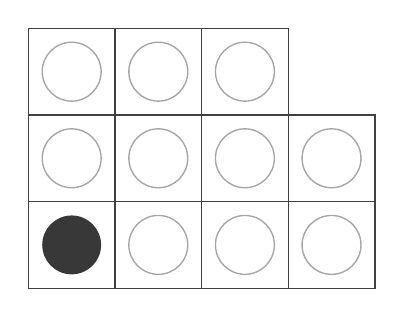
\begin{tikzpicture}[x=1mm, y=1mm]
\draw[line width=0.5pt, black!75] (0,0) rectangle ++(11,11);
\fill[black!78] (5.5,5.5) circle (3.74);
\draw[line width=0.5pt, black!75] (11,0) rectangle ++(11,11);
\draw[line width=0.5pt, black!35] (16.5,5.5) circle (3.74);
\draw[line width=0.5pt, black!75] (22,0) rectangle ++(11,11);
\draw[line width=0.5pt, black!35] (27.5,5.5) circle (3.74);
\draw[line width=0.5pt, black!75] (33,0) rectangle ++(11,11);
\draw[line width=0.5pt, black!35] (38.5,5.5) circle (3.74);
\draw[line width=0.5pt, black!75] (0,11) rectangle ++(11,11);
\draw[line width=0.5pt, black!35] (5.5,16.5) circle (3.74);
\draw[line width=0.5pt, black!75] (11,11) rectangle ++(11,11);
\draw[line width=0.5pt, black!35] (16.5,16.5) circle (3.74);
\draw[line width=0.5pt, black!75] (22,11) rectangle ++(11,11);
\draw[line width=0.5pt, black!35] (27.5,16.5) circle (3.74);
\draw[line width=0.5pt, black!75] (33,11) rectangle ++(11,11);
\draw[line width=0.5pt, black!35] (38.5,16.5) circle (3.74);
\draw[line width=0.5pt, black!75] (0,22) rectangle ++(11,11);
\draw[line width=0.5pt, black!35] (5.5,27.5) circle (3.74);
\draw[line width=0.5pt, black!75] (11,22) rectangle ++(11,11);
\draw[line width=0.5pt, black!35] (16.5,27.5) circle (3.74);
\draw[line width=0.5pt, black!75] (22,22) rectangle ++(11,11);
\draw[line width=0.5pt, black!35] (27.5,27.5) circle (3.74);
\end{tikzpicture}\par\vspace{10mm}
Is Ana right? Then explain which step of her reason breaks on this board, where the first player cannot make sure to win.\par\vspace{5mm}
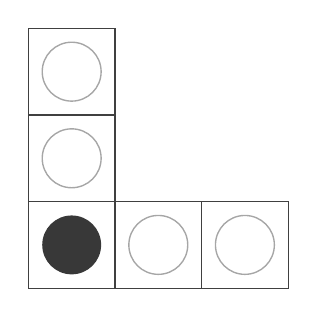
\begin{tikzpicture}[x=1mm, y=1mm]
\draw[line width=0.5pt, black!75] (0,0) rectangle ++(11,11);
\fill[black!78] (5.5,5.5) circle (3.74);
\draw[line width=0.5pt, black!75] (11,0) rectangle ++(11,11);
\draw[line width=0.5pt, black!35] (16.5,5.5) circle (3.74);
\draw[line width=0.5pt, black!75] (22,0) rectangle ++(11,11);
\draw[line width=0.5pt, black!35] (27.5,5.5) circle (3.74);
\draw[line width=0.5pt, black!75] (0,11) rectangle ++(11,11);
\draw[line width=0.5pt, black!35] (5.5,16.5) circle (3.74);
\draw[line width=0.5pt, black!75] (0,22) rectangle ++(11,11);
\draw[line width=0.5pt, black!35] (5.5,27.5) circle (3.74);
\end{tikzpicture}\par\vspace{0mm}
\newpage
\prob{7}Nobody knows a simple rule for finding a winning first bite on rectangles with three rows. On the 3 by 5 board and on this 3 by 6 board, mark a first bite after which the first player can make sure to win.\par\vspace{6mm}
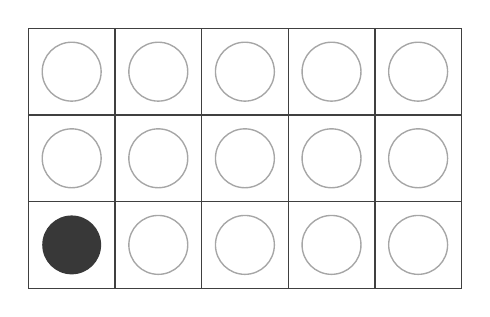
\begin{tikzpicture}[x=1mm, y=1mm]
\draw[line width=0.5pt, black!75] (0,0) rectangle ++(11,11);
\fill[black!78] (5.5,5.5) circle (3.74);
\draw[line width=0.5pt, black!75] (11,0) rectangle ++(11,11);
\draw[line width=0.5pt, black!35] (16.5,5.5) circle (3.74);
\draw[line width=0.5pt, black!75] (22,0) rectangle ++(11,11);
\draw[line width=0.5pt, black!35] (27.5,5.5) circle (3.74);
\draw[line width=0.5pt, black!75] (33,0) rectangle ++(11,11);
\draw[line width=0.5pt, black!35] (38.5,5.5) circle (3.74);
\draw[line width=0.5pt, black!75] (44,0) rectangle ++(11,11);
\draw[line width=0.5pt, black!35] (49.5,5.5) circle (3.74);
\draw[line width=0.5pt, black!75] (0,11) rectangle ++(11,11);
\draw[line width=0.5pt, black!35] (5.5,16.5) circle (3.74);
\draw[line width=0.5pt, black!75] (11,11) rectangle ++(11,11);
\draw[line width=0.5pt, black!35] (16.5,16.5) circle (3.74);
\draw[line width=0.5pt, black!75] (22,11) rectangle ++(11,11);
\draw[line width=0.5pt, black!35] (27.5,16.5) circle (3.74);
\draw[line width=0.5pt, black!75] (33,11) rectangle ++(11,11);
\draw[line width=0.5pt, black!35] (38.5,16.5) circle (3.74);
\draw[line width=0.5pt, black!75] (44,11) rectangle ++(11,11);
\draw[line width=0.5pt, black!35] (49.5,16.5) circle (3.74);
\draw[line width=0.5pt, black!75] (0,22) rectangle ++(11,11);
\draw[line width=0.5pt, black!35] (5.5,27.5) circle (3.74);
\draw[line width=0.5pt, black!75] (11,22) rectangle ++(11,11);
\draw[line width=0.5pt, black!35] (16.5,27.5) circle (3.74);
\draw[line width=0.5pt, black!75] (22,22) rectangle ++(11,11);
\draw[line width=0.5pt, black!35] (27.5,27.5) circle (3.74);
\draw[line width=0.5pt, black!75] (33,22) rectangle ++(11,11);
\draw[line width=0.5pt, black!35] (38.5,27.5) circle (3.74);
\draw[line width=0.5pt, black!75] (44,22) rectangle ++(11,11);
\draw[line width=0.5pt, black!35] (49.5,27.5) circle (3.74);
\end{tikzpicture}\par\vspace{14mm}
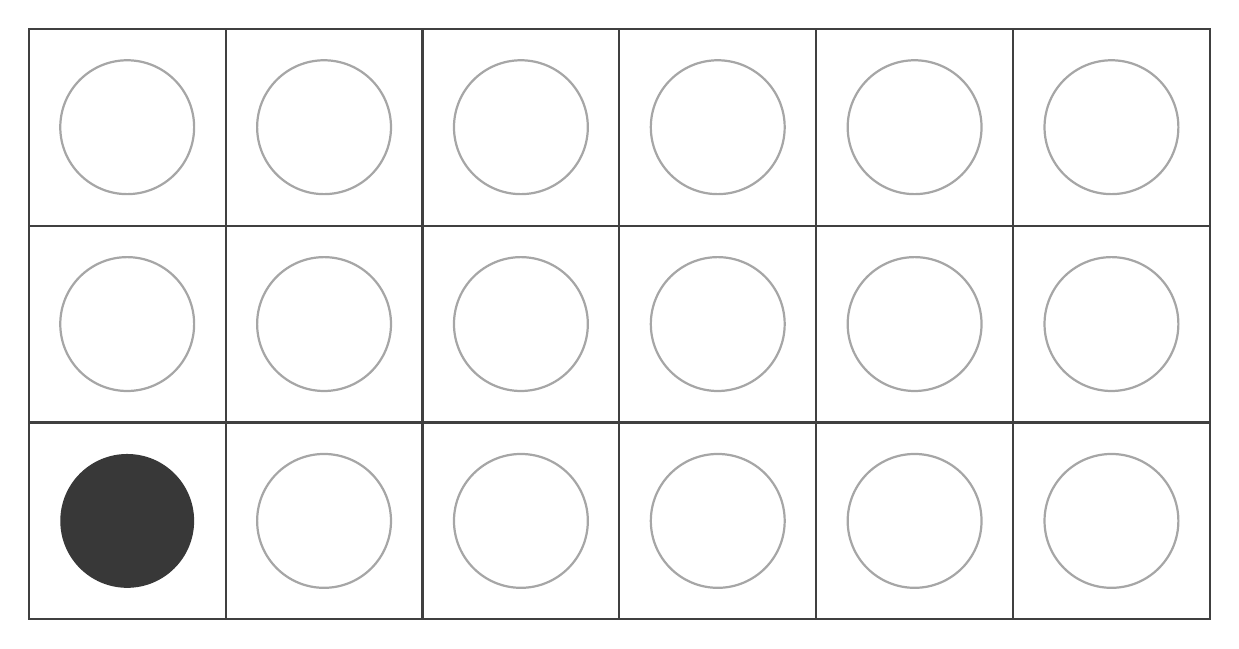
\begin{tikzpicture}[x=1mm, y=1mm]
\draw[line width=0.8pt, black!75] (0,0) rectangle ++(25,25);
\fill[black!78] (12.5,12.5) circle (8.5);
\draw[line width=0.8pt, black!75] (25,0) rectangle ++(25,25);
\draw[line width=0.8pt, black!35] (37.5,12.5) circle (8.5);
\draw[line width=0.8pt, black!75] (50,0) rectangle ++(25,25);
\draw[line width=0.8pt, black!35] (62.5,12.5) circle (8.5);
\draw[line width=0.8pt, black!75] (75,0) rectangle ++(25,25);
\draw[line width=0.8pt, black!35] (87.5,12.5) circle (8.5);
\draw[line width=0.8pt, black!75] (100,0) rectangle ++(25,25);
\draw[line width=0.8pt, black!35] (112.5,12.5) circle (8.5);
\draw[line width=0.8pt, black!75] (125,0) rectangle ++(25,25);
\draw[line width=0.8pt, black!35] (137.5,12.5) circle (8.5);
\draw[line width=0.8pt, black!75] (0,25) rectangle ++(25,25);
\draw[line width=0.8pt, black!35] (12.5,37.5) circle (8.5);
\draw[line width=0.8pt, black!75] (25,25) rectangle ++(25,25);
\draw[line width=0.8pt, black!35] (37.5,37.5) circle (8.5);
\draw[line width=0.8pt, black!75] (50,25) rectangle ++(25,25);
\draw[line width=0.8pt, black!35] (62.5,37.5) circle (8.5);
\draw[line width=0.8pt, black!75] (75,25) rectangle ++(25,25);
\draw[line width=0.8pt, black!35] (87.5,37.5) circle (8.5);
\draw[line width=0.8pt, black!75] (100,25) rectangle ++(25,25);
\draw[line width=0.8pt, black!35] (112.5,37.5) circle (8.5);
\draw[line width=0.8pt, black!75] (125,25) rectangle ++(25,25);
\draw[line width=0.8pt, black!35] (137.5,37.5) circle (8.5);
\draw[line width=0.8pt, black!75] (0,50) rectangle ++(25,25);
\draw[line width=0.8pt, black!35] (12.5,62.5) circle (8.5);
\draw[line width=0.8pt, black!75] (25,50) rectangle ++(25,25);
\draw[line width=0.8pt, black!35] (37.5,62.5) circle (8.5);
\draw[line width=0.8pt, black!75] (50,50) rectangle ++(25,25);
\draw[line width=0.8pt, black!35] (62.5,62.5) circle (8.5);
\draw[line width=0.8pt, black!75] (75,50) rectangle ++(25,25);
\draw[line width=0.8pt, black!35] (87.5,62.5) circle (8.5);
\draw[line width=0.8pt, black!75] (100,50) rectangle ++(25,25);
\draw[line width=0.8pt, black!35] (112.5,62.5) circle (8.5);
\draw[line width=0.8pt, black!75] (125,50) rectangle ++(25,25);
\draw[line width=0.8pt, black!35] (137.5,62.5) circle (8.5);
\end{tikzpicture}\par\vspace{0mm}

\end{document}
